% Original CCI-Class Controller — Project Roadmap
% Document ID: CCLI-ROADMAP-001  |  Revision 1.0
% Build: pdflatex CCI_Project_Roadmap.tex (×2 for TOC)

\documentclass[11pt,a4paper]{article}

\usepackage[T1]{fontenc}
\usepackage[utf8]{inputenc}
\usepackage{lmodern}
\usepackage{geometry}
\geometry{margin=22mm}

\usepackage{amsmath,amssymb}
\usepackage{booktabs}
\usepackage{array}
\usepackage{tabularx}
\usepackage{ragged2e}
\usepackage{hyperref}
\usepackage{xcolor}
\usepackage{graphicx}
\usepackage{enumitem}
\usepackage{fancyhdr}
\usepackage{eurosym}

\hypersetup{
  colorlinks=true,
  linkcolor=blue!60!black,
  citecolor=blue!60!black,
  urlcolor=blue!60!black,
  pdftitle={Original CCI-Class Controller Project Roadmap},
  pdfauthor={CCLI}
}

\definecolor{warnamber}{RGB}{180,83,9}
\definecolor{warnbg}{RGB}{255,251,235}
\definecolor{okgreen}{RGB}{22,101,52}
\definecolor{okbg}{RGB}{240,253,244}

\pagestyle{fancy}
\fancyhf{}
\fancyhead[L]{\small CCLI-ROADMAP-001 rev.\ 1.0}
\fancyhead[R]{\small CCI Project Roadmap}
\fancyfoot[C]{\thepage}
\renewcommand{\headrulewidth}{0.4pt}

\newcommand{\file}[1]{\texttt{#1}}
\newcommand{\docref}[1]{\textbf{#1}}

\title{%
  \textbf{Original CCI-Class Controller --- Project Roadmap}\\[0.4em]
  \large CEI~0-16 Annex~O/T/M compliant Central Plant Controller
}
\author{Document ID: CCLI-ROADMAP-001 \quad Revision: 1.0}
\date{2026-07-24}

\begin{document}
\maketitle
\thispagestyle{empty}

\begin{abstract}
\noindent
\textbf{Target:} CEI~0-16 Annex~O/T/M compliant Central Plant Controller, flexible 100\,kW--6\,MW MT plant range.\\
\textbf{Scope:} Original hardware/firmware design (not a clone of any existing commercial product).\\
\textbf{Prototype budget:} \textasciitilde{}\EUR{}1{,}000 (single unit, BOM + fab + assembly).\\
\textbf{Timeline stance:} Balanced --- solid working prototype in \textasciitilde{}10--12 weeks; grid/cyber certification is a separate, longer track.\\
\textbf{Existing certification:} organization already holds \textbf{ATEX} (EN/IEC~60079) --- reuse QMS, Notified Body relationship, and technical-file practice for the CEI~0-16 track below.\\
\textbf{Alternate track:} see companion brief \docref{CCLI-CLONE-RE-001} (\file{CCI\_Clone\_RE\_Option.pdf}) for the clone / reverse-engineering option, risks, and decision guide.
\end{abstract}

\begin{center}
\begin{minipage}{0.95\linewidth}
\colorbox{okbg}{%
  \parbox{\dimexpr\linewidth-2\fboxsep\relax}{%
    \small
    \textbf{\textcolor{okgreen}{Already in place:}}
    your company is \textbf{ATEX-certified} (EN/IEC~60079 product family experience).
    That is a real head start --- technical files, NB engagement, and production QA patterns do not start from zero.
    Standard MT CCI cabinet installations are usually \emph{non-hazardous area}; confirm per project whether Ex marking is required on the CCI itself.
  }%
}
\end{minipage}
\end{center}

\vspace{0.5em}
\begin{center}
\begin{minipage}{0.95\linewidth}
\colorbox{warnbg}{%
  \parbox{\dimexpr\linewidth-2\fboxsep\relax}{%
    \small
    \textbf{\textcolor{warnamber}{Set expectations up front:}}
    the hardware prototype is the \emph{cheap and fast} part of this project.
    Certification still required for this product class (IEC~62443-4-1/4-2, IEC~61850 conformance, IEC~62351, CEI~0-16 demonstration) ---
    realistically \EUR{}50{,}000--120{,}000+ and 9--18 months for the \emph{remaining} grid/cyber scope.
    ATEX is already held and is not budgeted again here.
  }%
}
\end{minipage}
\end{center}

\tableofcontents
\newpage

%==============================================================================
\section{System architecture (original design)}
%==============================================================================

This block diagram reflects the \emph{generic, publicly-documented functional interfaces} that CEI~0-16 Annexes~O/T
require of any CCI (dual DSO/Operator Ethernet separation, plant-side ports, serial link to the energy analyzer,
time sync, DI/DO for status/command) --- not any specific vendor's schematic or component selection.
Figure~\ref{fig:architecture} shows the visual companion to this section.

\begin{figure}[htbp]
\centering
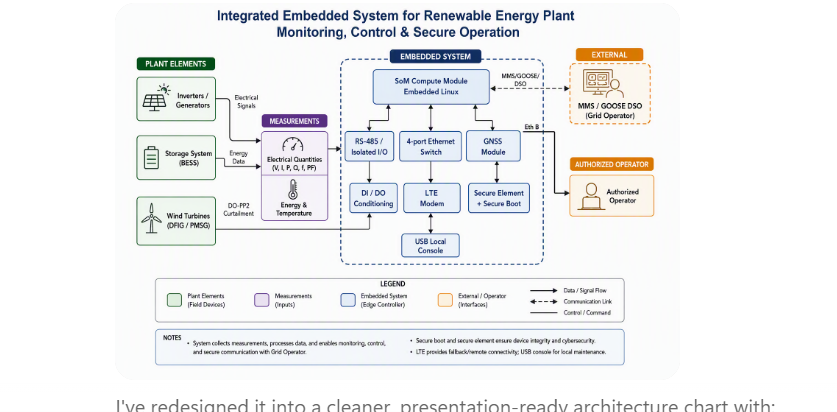
\includegraphics[width=\linewidth]{CCI_Architecture.png}
\caption{CCI system architecture --- integrated embedded edge controller for renewable plant monitoring, control, and secure DSO/operator communication (CEI~0-16 Annexes~O/T functional view)}
\label{fig:architecture}
\end{figure}

\subsection{Core functional blocks}

\begin{table}[htbp]
\centering
\caption{Core functional blocks and design-track assignment}
\label{tab:core-blocks}
\renewcommand{\arraystretch}{1.15}
\small
\begin{tabularx}{\linewidth}{@{}>{\raggedright\arraybackslash}p{2.65cm}>{\raggedright\arraybackslash}p{5.4cm}>{\RaggedRight\arraybackslash}X@{}}
\toprule
\textbf{Block} & \textbf{Function} & \textbf{Notes / track} \\
\midrule
Design approach &
Option~A (default): original SoM + carrier derived from public CEI~0-16 Annex~O/T interfaces &
Primary track for this roadmap. Independent schematic, layout, and firmware boundary. \\
\addlinespace
Design approach &
Option~B: clone via reverse engineering of a commercial CCI (AiLux-class reference) &
Separate brief \docref{CCLI-CLONE-RE-001} (\file{CCI\_Clone\_RE\_Option.pdf}). Higher IP/legal and certification risk; use only as a gated research spike, not the default product path. \\
\midrule
Compute module (SoM) &
Runs embedded Linux, IEC~61850 server, Modbus master, PF2 control logic &
Option~A: Toradex/Variscite/Compulab-class SoM. See \S\ref{sec:som}. Option~B: match reference compute block only if legally cleared. \\
Ethernet interfaces ($\geq$4-port managed switch or SoM+switch IC) &
Eth\_A $\rightarrow$ DSO (isolated, FO-ready via external media converter); Eth\_B $\rightarrow$ authorized Operator; 2$\times$ plant-facing ports &
Functional requirement: physical/electrical separation between DSO and plant networks --- minimum two isolated PHYs/VLANs. Do not copy vendor PHY placement verbatim on Option~B. \\
RS-485/RS-232 serial ($\times$2, isolated) &
Modbus RTU master to energy analyzer (Ax M22/MT1-class); IEC~60870-5-101 optional &
Opto-isolated transceivers, switchable termination. Map registers from analyzer datasheet, not from copied reference firmware. \\
GNSS module &
Time sync for timestamped measurements and events &
Standard u-blox-class module with passive/active antenna. Commodity block on both tracks. \\
Cellular modem (LTE Cat-1/Cat-4) &
Remote configuration, monitoring, and backup communications &
Optional on rev~A if DSO link is wired. Modular socket; omit from first prototype if not needed. \\
Digital I/O &
DI: polarized/optoisolated 10--120\,Vdc status inputs; DO: dry contact for command/curtailment relay &
Critical PF2 actuation path. Option~A: design from CEI limits. Option~B: observe reference thresholds only; re-implement conditioning network. \\
Secure element + secure boot &
Root of trust, key storage, and signed firmware &
Option~A: ATECC608B/STSAFE-A110-class parts with your own key hierarchy. Option~B: do not extract or reuse reference keys/boot chain. \\
Local console &
USB service port for commissioning and diagnostics &
Outside certified control path on both tracks; web/Python tooling acceptable here. \\
Power input &
12--24\,Vdc wide-range isolated DC-DC &
Typical Box CCI UPS/battery context. Size from SoM + field I/O budget; standard off-the-shelf power module. \\
\bottomrule
\end{tabularx}
\end{table}

%==============================================================================
\section{Compute module: SoM + custom carrier}
\label{sec:som}
%==============================================================================

\textbf{Decision (from our discussion):} off-the-shelf industrial SoM, original carrier board design.

Candidate SoM families to evaluate (pick based on Linux BSP maturity, industrial temp range, and 10-year longevity
commitment --- you need this for a utility-facing product):

\begin{itemize}[noitemsep]
  \item Toradex Verdin iMX8M Mini/Plus
  \item Variscite DART-MX8M-Mini / DART-MX8M-Plus
  \item Compulab CL-SOM-iMX8
  \item NXP i.MX8M Mini EVK-class reference designs
\end{itemize}

All of these ship a maintained Yocto BSP, handle DDR/power-sequencing/thermal internally, and let your carrier board
stay a straightforward 2--4 layer design (Ethernet PHYs, RS-485 transceivers, GNSS/LTE module sockets, DI/DO conditioning, power).

%==============================================================================
\section{Prototype BOM target (single unit, \textasciitilde{}\EUR{}1{,}000)}
%==============================================================================

\begin{tabularx}{\linewidth}{@{}l>{\raggedright\arraybackslash}X>{\raggedright\arraybackslash}X@{}}
\toprule
\textbf{Item} & \textbf{Est.\ cost (EUR)} & \textbf{Notes} \\
\midrule
Industrial SoM (qty 1) & \EUR{}60--120 & Toradex/Variscite-class, i.MX8M Mini tier \\
Carrier PCB fab (4-layer, small batch 5--10 pcs) & \EUR{}50--150 & JLCPCB/PCBWay prototype tier \\
Assembly (self or light-touch SMT service) & \EUR{}100--250 & BGA stays on the SoM module --- carrier assembly is hand/reflow-feasible \\
Ethernet PHYs/magnetics/RJ45 ($\times$4) & \EUR{}15--25 & \\
RS-485/RS-232 isolated transceivers ($\times$2) & \EUR{}10--15 & \\
GNSS module + antenna & \EUR{}25--40 & u-blox-class \\
LTE module + antenna + SIM holder & \EUR{}25--40 & Quectel-class; optional on rev~A \\
Secure element & \EUR{}2--5 & e.g.\ Microchip ATECC608B / STSAFE-A110 class part \\
DI/DO conditioning (opto-isolators, relays) & \EUR{}15--25 & \\
Power stage (wide-range isolated DC-DC) & \EUR{}15--25 & \\
DIN rail hardware, connectors, terminal blocks, enclosure & \EUR{}40--60 & \\
Passives, stencil, shipping, contingency & \EUR{}80--150 & \\
\midrule
\textbf{Total (single prototype)} & \textbf{\textasciitilde{}\EUR{}440--900} & Leaves headroom within \EUR{}1{,}000 for one respin's worth of parts \\
\bottomrule
\end{tabularx}

\vspace{0.75em}
\noindent
This is a \emph{component-cost} estimate for one unit at prototype quantities --- not a manufactured unit cost at volume,
which would drop significantly (likely \EUR{}150--300/unit at 100+ qty once NRE is amortized).

%==============================================================================
\section{Path to Gerbers}
%==============================================================================

\begin{table}[htbp]
\centering
\caption{Carrier board workflow --- Altium Designer to prototype fab}
\label{tab:path-to-gerbers}
\renewcommand{\arraystretch}{1.12}
\small
\begin{tabularx}{\linewidth}{@{}c>{\raggedright\arraybackslash}p{2.4cm}>{\RaggedRight\arraybackslash}X@{}}
\toprule
\textbf{\#} & \textbf{Step} & \textbf{Activity (Altium Designer)} \\
\midrule
1 & Architecture freeze &
Lock interfaces, connector count, and power budget before opening the project --- changes after layout start cost a full re-pass. \\
2 & Schematic capture &
Capture in \textbf{Altium Designer} from datasheets and your interface decisions. Link SoM/PHY/transceiver symbols to verified footprints early. \\
3 & Design review &
Checklist pass: power sequencing vs SoM requirements; ESD/surge on every field I/O (RS-485, DI/DO, Ethernet); isolation barriers where required. \\
4 & PCB layout &
Place SoM footprint first (follow vendor carrier guide), then Ethernet PHY/magnetics, then RS-485, power, and RF/LTE. Keep analog/field wiring away from switching nodes. \\
5 & DFM check &
Run Altium DRC, then the target fab's DFM portal (JLCPCB/PCBWay) against fab stackup and drill rules before order. \\
6 & Fab outputs &
Generate via Altium \textbf{Output Job}: Gerber RS-274X, NC drill, IPC-2581 or ODB++ if requested, assembly pick-and-place, and BOM (ActiveBOM or structured export). \\
7 & Fab + assembly &
1--3 week turnaround typical at prototype scale; hand or SMT assembly on carrier only (BGA stays on SoM). \\
8 & Bring-up &
Power-on test, boot SoM, verify each interface individually (Ethernet $\times$4, RS-485 $\times$2, GNSS, LTE, DI/DO) before firmware integration. \\
\bottomrule
\end{tabularx}
\end{table}

%==============================================================================
\section{Firmware architecture \& language choice}
%==============================================================================

\begin{itemize}[leftmargin=*]
  \item \textbf{OS/BSP:} Yocto-based embedded Linux (matches SoM vendor's supported BSP) --- gives you package management,
        OTA update tooling, and a known-good foundation auditors are familiar with.
  \item \textbf{Core control/protocol path} (IEC~61850 server, Modbus master, PF2 curtailment logic, GOOSE handling):
        C/C++. This is the code that will eventually face conformance and security audits --- auditors and test labs are far
        more comfortable reviewing statically-typed, analyzable C/C++ than dynamic scripting languages, and real-time GOOSE
        timing requirements favor it anyway.
  \item \textbf{Config/commissioning tooling, local web console, diagnostics:} Python or a lightweight web stack is fine here ---
        this code is outside the certified control-path boundary, so language choice is a productivity call, not a compliance one.
        Keep the boundary between ``certified path'' and ``tooling'' architecturally clean from day one --- it makes scoping the
        IEC~62443-4-2 assessment much cheaper later.
  \item \textbf{IEC~61850 stack:} start on \textbf{libiec61850} (MZ Automation, \textbf{GPLv3}) for prototype/demo
  (MMS/GOOSE/SV/R-Session). Commercial licenses sold separately by MZ Automation for shipping a closed product ---
  treat OSS as \emph{free to prototype, pay to ship}; budget the commercial license from day one.
  Evaluate commercial stacks (SISCO, Triangle MicroWorks) before paid conformance testing --- see \S\ref{sec:cert}.
  \item \textbf{Security baseline to build in from day one} (cheap now, expensive to retrofit later): secure boot chain, signed
        firmware images, TLS/DTLS for IEC~62351, key storage in the secure element, basic RBAC on the local console, audit logging.
        IEC~62443-4-1 specifically audits \emph{how} you built and maintain the product (your SDLC), not just what features it has ---
        so start documenting your development process now, not after the fact.
\end{itemize}

%==============================================================================
\section{Timeline --- Phase 1: Hardware + firmware prototype (\textasciitilde{}10--12 weeks)}
%==============================================================================

\begin{tabularx}{\linewidth}{@{}lX@{}}
\toprule
\textbf{Weeks} & \textbf{Milestone} \\
\midrule
1--2 & Architecture freeze, SoM selection finalized, schematic capture starts \\
2--4 & Schematic complete + design review, long-lead parts ordered (SoM, LTE/GNSS modules) \\
4--6 & PCB layout, DFM check, Gerbers to fab \\
6--8 & Fab + assembly turnaround \\
8--10 & Hardware bring-up: power, boot, verify each interface (Ethernet $\times$4, RS-485 $\times$2, GNSS, LTE, DI/DO) \\
10--12 & Firmware integration: libiec61850 server running, Modbus master polling a real analyzer, DO-driven curtailment stub, local console reachable \\
\bottomrule
\end{tabularx}

\vspace{0.75em}
\noindent
\textbf{Exit criteria for this phase:} a DIN-rail prototype that boots reliably, exposes an IEC~61850 MMS server over Eth\_A,
polls a Modbus energy analyzer over RS-485, timestamps data via GNSS, and can toggle a DO relay from a simulated DSO command.
This is a credible demo/investor/pilot-partner artifact --- it is \emph{not} yet field-deployable at a real MT POC.

%==============================================================================
\section{Phase 2: Certification path (separate track, 9--18 months)}
\label{sec:cert}
%==============================================================================

\noindent
\textbf{Scope note:} ATEX (EN/IEC~60079) is \textbf{already certified} for the organization --- treat it as established capability, not a new line item.
Phase~2 below covers the \emph{remaining} CEI~0-16 / grid-interface / cybersecurity workstreams for this CCI product.

\begin{table}[htbp]
\centering
\caption{Certification workstreams --- remaining scope (ATEX already held)}
\label{tab:cert-path}
\renewcommand{\arraystretch}{1.12}
\small
\begin{tabularx}{\linewidth}{@{}>{\raggedright\arraybackslash}p{3.1cm}>{\RaggedRight\arraybackslash}X>{\raggedright\arraybackslash}p{2.3cm}>{\raggedright\arraybackslash}p{2.3cm}@{}}
\toprule
\textbf{Workstream} & \textbf{What it involves} & \textbf{Rough cost} & \textbf{Duration} \\
\midrule
ATEX (EN/IEC~60079) &
\textbf{Already held} --- existing org certification, NB relationship, and hazardous-area design process &
Sunk / reuse &
--- \\
IEC~62443-4-1 (Secure SDLC) &
Process audit of secure development lifecycle. Partial overlap with ATEX QMS/documentation habits, but cyber-specific artifacts still required &
\EUR{}10{,}000--30{,}000 &
2--5 months \\
IEC~62443-4-2 (device security) &
Lab test vs SL1 (CEI~0-16 FAQ minimum), target SL2 capability &
\EUR{}15{,}000--40{,}000 &
2--4 months \\
IEC~61850 conformance &
Accredited lab (DNV/KEMA, OMICRON, Kalkitech-class) validates MMS/GOOSE/reporting &
\EUR{}10{,}000--25{,}000 &
1--3 months \\
IEC~62351 protocol testing &
Cybersecurity protocol testing; scarce lab capacity --- schedule slack &
Overlaps 4-2 &
3--6 months \\
CEI~0-16 Annex~O/T + DSO demo &
Functional observability / PF2 exchange with DSO or recognized test environment &
Integrator time &
1--3 months \\
\bottomrule
\end{tabularx}
\end{table}

\vspace{0.75em}
\noindent
\textbf{All-in realistic budget for first CEI-class CCI certification: roughly \EUR{}45{,}000--110{,}000, spread over 9--18 months} (ATEX excluded --- already held).
This is the real reason the commercial Italian CCIs (AiLux, Selta, Energy Team, Higeco) price the way they do --- you're not
paying for a \EUR{}400 BOM, you're amortizing exactly this certification investment across thousands of installed units.
Your path to being genuinely cheaper is either (a)~volume --- this cost amortizes the same way once you're past unit 50--100 --- or
(b)~a leaner process by scoping the 62443-4-2 boundary tightly around just the certified control path (see the firmware architecture
note in \S5), which measurably shrinks lab scope and cost.

%==============================================================================
\section{Team/skills needed}
%==============================================================================

\begin{itemize}[noitemsep]
  \item Embedded hardware engineer (schematic + layout, comfortable with SoM carrier design)
  \item Embedded Linux/firmware engineer (Yocto, C/C++, protocol stacks)
  \item Someone who can own the IEC~62443-4-1 process documentation --- can leverage existing ATEX technical-file and NB workflow experience
  \item A relationship with an accredited test lab early --- your ATEX Notified Body may also offer or partner on 62443/61850 scoping
\end{itemize}

%==============================================================================
\section{Immediate next steps}
%==============================================================================

\begin{enumerate}[leftmargin=*]
  \item Confirm SoM family choice (Toradex vs Variscite vs Compulab) based on your BSP/tooling comfort and long-term sourcing preference.
  \item Draft the interface list and pin budget (connector-by-connector) as a starting schematic outline --- original to your design,
        not copied from any existing product.
  \item Get a scoping quote from one IEC~62443/61850 test lab now, even before hardware exists --- their capacity and requirements should
        shape your firmware architecture decisions, not the other way around.
\end{enumerate}

\end{document}
